\documentclass[12pt]{report}

\usepackage{commands}


\begin{document}

\large

\begin{center}
 Math 586 Homework 1\\
 Due April 10 11pm\\
 By Marvyn Bailly\\
\end{center}

\normalsize

\hrule



%---------------%
%---Problem 1---%
%---------------%

%--status--$

\begin{problem}
    In this exercise you will show convergence for a discretization of
  \begin{align*}
    \begin{cases}
      -u''(x) = g(x),\\
      u'(0) = \alpha,\\
      u(1) = \beta.
    \end{cases}
  \end{align*}
  \begin{enumerate}
\item  Consider the $(m+1) \times (m+1)$ matrix
  \begin{align*}
    A = \begin{bmatrix} 1 & -1 \\ -1 & 2 &-1 \\
    & \ddots & \ddots & \ddots \\
    &&&& -1\\
    &&&-1& 2\\
  \end{bmatrix}.
    \end{align*}
    Find its Cholesky decomposition.
  \item Show that
    \begin{align}\label{unit} A^{-1} \begin{bmatrix}  1 \\ 0 \\ \vdots \\ 0 \end{bmatrix} = \begin{bmatrix}  m +1 \\ m \\ \vdots \\ 1 \end{bmatrix}.\end{align}
  \item Now show that
    \begin{align*}
      \|A^{-1}\|_1 \leq (m+1)^2, \quad \|A^{-1}\|_\infty \leq (m+1)^2.
    \end{align*}
  \end{enumerate}
\end{problem}

\begin{solution}
    \noindent
    \begin{enumerate}
      \item [(a)]
      We wish to find the Cholesky decomposition of the $(m+1) \times (m+1)$ matrix
      \begin{align*}
        A = \begin{bmatrix} 
          1 & -1 \\ -1 & 2 &-1 \\
        & \ddots & \ddots & \ddots \\
        &&&& -1\\
          &&&-1& 2\\
        \end{bmatrix}.
      \end{align*}
      Since $A$ is an HPD, there exists a unique Cholesky decomposition $L$ such that $A = LL^*$. We can find $L$ by preforming Gaussian Elimination on $A$ and collecting the row operations in the a matrix $L$. The first step of Gaussian Elimination looks like
      \begin{align*}
        A = \begin{bmatrix} 1 & -1 \\ -1 & 2 &-1 \\
          & \ddots & \ddots & \ddots \\
          &&&& -1\\
          &&&-1& 2\\
        \end{bmatrix} \xrightarrow{r_1 + r_{2} \rightarrow r_{2}} \begin{bmatrix} 1 & -1 \\ 0 & 1 &-1 \\
          & \ddots & \ddots & \ddots \\
          &&&& -1\\
          &&&-1& 2\\
        \end{bmatrix},
      \end{align*}
      where $L_1$ is given by
      \begin{align*}
        L_1 = \begin{bmatrix}
          1 & \\
          1 & 1\\
          && \ddots\\
          &&&1
        \end{bmatrix}.
      \end{align*}
      Continuing this process of adding the $i$th row to the $i+1$th row gives
      \begin{align*}
        \begin{bmatrix} 1 & -1 \\ 0 & 1 &-1 \\
          & \ddots & \ddots & \ddots \\
          &&&& -1\\
          &&&-1& 2\\
        \end{bmatrix} \rightarrow 
        \begin{bmatrix} 
          1 & -1 \\ 
          0 & 1 &-1 \\
          & \ddots & \ddots & \ddots \\
          &&&& -1\\
          &&&0& 1\\
        \end{bmatrix} = U.
      \end{align*} 
      Thus we have found that
      \begin{align*}
        (L_{m} \cdots L_1) A = U.
      \end{align*}
      Then we define the Cholesky Factorization as 
      \begin{align*}
        L = (L_{m} \cdots L_1)^{-1} = \begin{bmatrix} 1 \\ -1 & 1 \\
          & \ddots & \ddots \\
          &&&&\\
          &&&-1& 1\\
        \end{bmatrix} = \begin{bmatrix} 
          1 \\ 
          -d_1 & 1 \\
          & \ddots & \ddots \\
          &&&&\\
          &&&-d_{m}& 1\\
        \end{bmatrix},
      \end{align*}
      where $A = LL^*$.

      \item [(b)]
      Next we wish to show that
      \begin{align*}\label{unit} A^{-1} \begin{bmatrix}  1 \\ 0 \\ \vdots \\ 0 \end{bmatrix} = \begin{bmatrix}  m +1 \\ m \\ \vdots \\ 1 \end{bmatrix} \implies A \begin{bmatrix}  m +1 \\ m \\ \vdots \\ 1 \end{bmatrix} = \begin{bmatrix}  1 \\ 0 \\ \vdots \\ 0 \end{bmatrix}.\end{align*}
      Observe that 
      \begin{align*}
        \begin{bmatrix} 1 & -1 \\ -1 & 2 &-1 \\
          & \ddots & \ddots & \ddots \\
          &&&& -1\\
          &&&-1& 2\\
        \end{bmatrix}\begin{bmatrix}  m +1 \\ m \\ \vdots \\ 1 \end{bmatrix}  = \begin{bmatrix}
          m + 1 - m + 0\\
          - m - 1 + 2m - m + 1 + 0\\
          \vdots\\
          0 + 2 - 2
        \end{bmatrix} = \begin{bmatrix}
          1\\ 0 \\ \vdots \\ 0
        \end{bmatrix}.
      \end{align*}

      \item [(c)]
      Now we wish to show that 
      \begin{align*}
        \|A^{-1}\|_1 \leq (m+1)^2, \quad \|A^{-1}\|_\infty \leq (m+1)^2.
      \end{align*}
      Since $A$ is HPD, $A^{-1}$ is as well. This means that $\|A^{-1}\|_1 = \|A^{-1}\|_\infty$ due to symmetry. Observe that
      \begin{align*}
        \|A^{-1}\|_\infty = \|A^{-1}\|_1 &\leq \| L^{-*} \|_1 \| L^{-1} \|_1\\
         &= \paren{1 + \max_{2 \leq + i \leq m} \sum^m_{j = i +1} \prod_{l = i}^{j} |d_l|}\paren{1 + \max_{2 \leq + i \leq m} \sum^{j-1}_{i = 1} \prod_{l = i}^{j} |d_l|}\\
         &\leq (1 + m)(1 + m)\\
        &= (1 + m)^2.
      \end{align*}


    \end{enumerate}
\end{solution}

%----------------------------------------------------------------------------------------------------%
%\vskip 20pt
\newpage

%---------------%
%---Problem 2---%
%---------------%

%--status--$

\begin{problem}
    Consider the matrix (see (2.54) in LeVeque)
    \begin{align*}
      L = h^{-2} \begin{bmatrix} h & -h \\ -1 & 2 &-1 \\  
    & \ddots & \ddots & \ddots \\
    &&&& -1\\
    &&&-1& 2\\
  \end{bmatrix}.\end{align*}
\begin{enumerate}
  \item Compute $L^{-1}$ in terms of $A^{-1}$ and compute bounds for  $\|L^{-1}\|_1$ and $\|L^{-1}\|_\infty$.
  \item Explain why this is not enough to imply convergence for the one-sided approach, (2.53) in LeVeque.
    \item Use \eqref{unit} to show the method converges in both the grid 1-norm and the $\infty$-norm.
  \end{enumerate}
\end{problem}

\begin{solution}
  
    \noindent
    Consider the matrix
    \begin{align*}
      L = h^{-2} 
      \begin{bmatrix} 
        h & -h \\ -1 & 2 &-1 \\  
        & \ddots & \ddots & \ddots \\
        &&&& -1\\
        &&&-1& 2\\
  \end{bmatrix}.\end{align*}
  \begin{enumerate}
    \item [(a)]
      We first wish to compute $L^{-1}$ is terms of $A^{-1}$. Observe that 
      \begin{align*}
        L = \frac{1}{h^2} \begin{bmatrix}
          h\\
          &1\\
          &&\ddots\\
          &&&1
        \end{bmatrix} A = \frac{1}{h^2}BA,
      \end{align*}
      and thus we have that
      \begin{align*}
        L^{-1} = \paren{\frac{1}{h^2}AB}^{-1} = h^2A^{-1}B^{-1}.
      \end{align*}
      Next we can bound $\|L^{-1}\|_1$ by observing 
      \begin{align*}
        \| L^{-1} \|_1 &= h^2 \|A^{-1}B^{-1}\|_1\\
          &= h^2\|A^{-1}\|_1\|B^{-1}\|_1\\
          &= h^2 (m+1)^2 \left|\frac{1}{h}\right|\\
          &= h(m+1)^2\\
          &= m+1 = h^{-1}.
      \end{align*}
      Next we wish to bound $\|L^{-1}\|_\infty = h^2 \|A^{-1}B^{-1}\|_\infty \leq h^2\|A^{-1}\|_\infty\|B^{-1}\|_\infty$. We know that $\|A^{-1}\|_1 = \|A^{-1}\|_\infty$ and since $B$ is symmetric, we know that $B^{-1}$ is also symmetric and thus $\|B^{-1}\|_1 = \|B^{-1}\|_\infty$. Therefore we have that $\|L^{-1}\|_\infty \leq h^{-1}$.



    \item [(b)]
    To see why this bound is not strong enough to imply convergence for the one-sided approach presented in LeVeque, observe the following. Let $E_j = u(x_j) - u_j$, then we have that
    \[
      L[E_j] = \begin{bmatrix}
        h u''(\xi_0)/2\\
        h^2 u''''(\xi_1)/12\\
        \vdots\\
        h^2 u''''(\xi_m)/12
      \end{bmatrix} = \begin{bmatrix}
        O(h)\\
        O(h^2)\\
        \vdots\\
        O(h^2)
      \end{bmatrix}
    \]
    Thus we see that
    \begin{align*}
      \|[E_j]\|_1 &= \left\| L^{-1} \cdot \begin{bmatrix}
        h u''(\xi_0)/2\\
        h^2 u''''(\xi_1)/12\\
        \vdots\\
        h^2 u''''(\xi_m)/12
      \end{bmatrix}\right\|_1\\
      &\leq \| L^{-1}\|_1 \cdot \left\| \begin{bmatrix}
        h u''(\xi_0)/2\\
        h^2 u''''(\xi_1)/12\\
        \vdots\\
        h^2 u''''(\xi_m)/12
      \end{bmatrix}\right\|_1\\
      &\leq \left\| \begin{bmatrix}
        u''(\xi_0)/2\\
        h u''''(\xi_1)/12\\
        \vdots\\
        h u''''(\xi_m)/12
      \end{bmatrix}\right\|_1\\
      &\leq \frac{\|u''\|_\infty}{2}.
    \end{align*} 
    Thus we see that the method is not necessarily consistent as $\|[E_j]\|_1$ does not have to go to zero as $h \to \infty$. Therefore, the bound on $\|L\|_1$ is not sufficient to guarantee convergence. A similar result occurs when studying $\|[E_j]\|_\infty$. 

    \item [(c)]
    To show the method converges in both the grid $1$-norm and the $\infty$-norm, recall that convergence in the $\infty$-norm implies convergence in the $1$-norm. Thus let's find a stricter bound on the $\infty$-norm that shows the method is consistent and thus convergences. Recall that in part one we found
    \[ 
      L^{-1} = h^2 A^{-1}B^{-1} \implies A^{-1} = \frac{1}{h^2}L^{-1}B,
    \]
    where
    \[ 
      B = \begin{bmatrix}
        h\\ &1\\ &&\ddots\\ &&&1
      \end{bmatrix}.
    \]
    Then we have that
    \begin{align*}
      [E_j] &= L^{-1}\\
      &=  L^{-1}\begin{bmatrix}
        h u''(\xi_0)/2\\
        h^2 u''''(\xi_1)/12\\
        \vdots\\
        h^2 u''''(\xi_m)/12
      \end{bmatrix}\\
      &= h^2 A^{-1}B^{-1} \begin{bmatrix}
        h u''(\xi_0)/2\\
        h^2 u''''(\xi_1)/12\\
        \vdots\\
        h^2 u''''(\xi_m)/12
      \end{bmatrix}\\
      &= - h^2A^{-1} \begin{bmatrix}
        u''(\xi_0)/2\\
        h^2 u''''(\xi_1)/12\\
        \vdots\\
        h^2 u''''(\xi_m)/12
      \end{bmatrix}\\
      &= - \frac{h^2 u''(\xi_0)}{2}A^{-1}\begin{bmatrix}
        1\\ 0 \\ \vdots \\ 0
      \end{bmatrix} - \frac{h^2}{12}A^{-1}\begin{bmatrix}
        0\\ h^2 u''''(\xi_1) \\ \vdots\\ h^2 u''''(\xi_m)
      \end{bmatrix}\\
      &= - \frac{h^2 u''(\xi_0)}{2}\begin{bmatrix}
        m+1\\ m \\ \vdots \\ 1
      \end{bmatrix} - \frac{h^4}{12}A^{-1}\begin{bmatrix}
        0\\ u''''(\xi_1) \\ \vdots\\  u''''(\xi_m)
      \end{bmatrix}.\\
    \end{align*}
    Then applying the grid $\infty$-norm yields
    \begin{align*}
      \|[E_j]\|_\infty &\leq \frac{\|u''\|_\infty}{2} h^2 (m+1) + \frac{\|u''''\|_\infty}{12} h^4(m+1)^2\\
      &= O(h) + O(h^2).
    \end{align*}
    Thus we have that that $\|[E_j]\|_\infty$ is consistent since $\|[E_j]\|_\infty \rightarrow 0$ as $h\rightarrow 0$. Thus the method converges under the grid $\infty$-norm which means that the method also converges under the grid one-norm (as $\| [E_j] \|_1 \leq \| [E_j] \|_\infty$ ). 

  \end{enumerate}
\end{solution}

%----------------------------------------------------------------------------------------------------%
%\vskip 20pt
\newpage

%---------------%
%---Problem 1---%
%---------------%

%--status--$

\begin{problem}
    Consider $u(x) = \cos(k \pi x) \exp(-x^2)$.  Determine $g$, $\alpha$ and $\beta$ such that
  \begin{align*}
    \begin{cases} -u''(x) = g(x),\\
      u(0) = \alpha,\\
      u(1) = \beta. \end{cases}
  \end{align*}
  \begin{enumerate}
  \item Modify the code in {\tt LinearBVP.ipynb} to solve this BVP using a second-order accurate method.  Plot errors on a log-log scale for $k = 1,2,3,4$.
   \item Modify the code in {\tt LinearBVP.ipynb} to solve this BVP using a fifth-order accurate method.  Plot errors on a log-log scale for $k = 1,2,3,4$. 
  \end{enumerate}
\end{problem}

\begin{solution}

    \noindent
    \begin{enumerate}
      \item [(a)]
      
      \begin{figure}[h!]
        \centering
        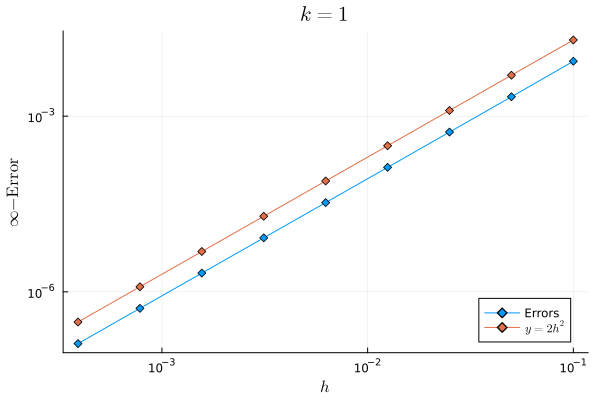
\includegraphics[width=0.48\linewidth]{images/1a1.png}
        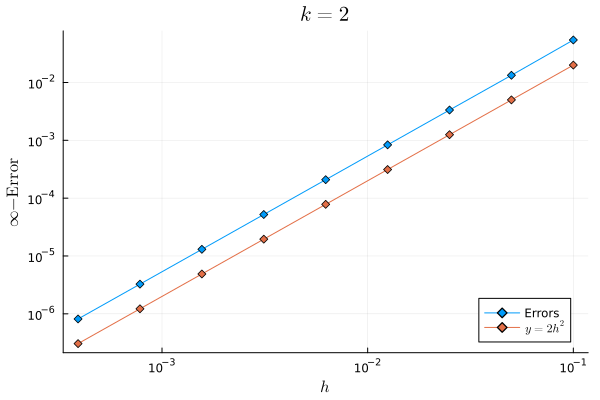
\includegraphics[width=0.48\linewidth]{images/2a1.png}
        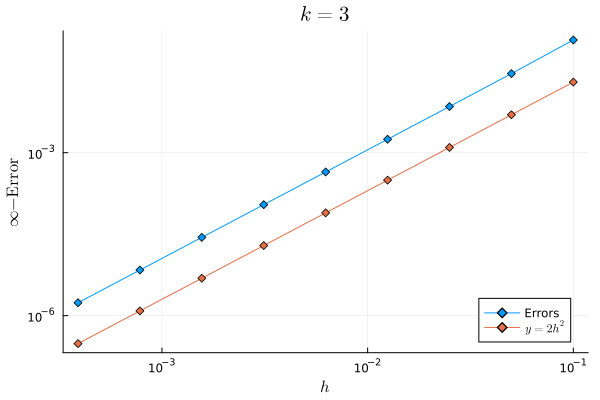
\includegraphics[width=0.48\linewidth]{images/3a1.png}
        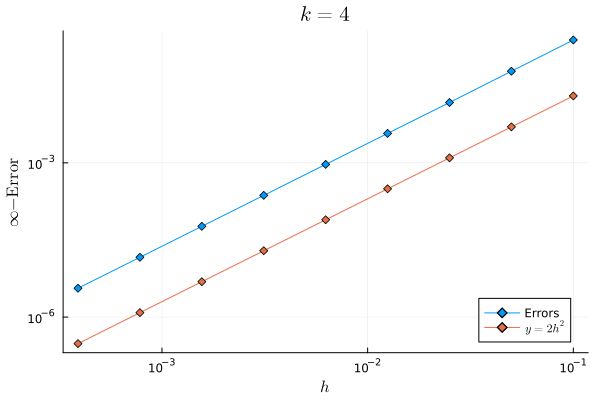
\includegraphics[width=0.48\linewidth]{images/4a1.png}
        \caption{Loglog plots of errors using a second-order accurate method for $k \in \{1,2,3,4\}$ compare to a line of slope $h^2$.}
      \end{figure}

      From Figure 1 we can see that the slope of error for reducing grid sizes for $k \in \{1,2,3,4\}$ is order $h^2$ as expected. 

      \item [(b)]
      
      \begin{figure}[H]
        \centering
        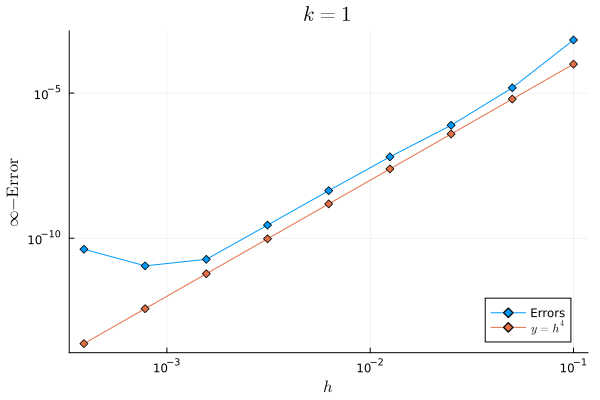
\includegraphics[width=0.48\linewidth]{images/1b1.png}
        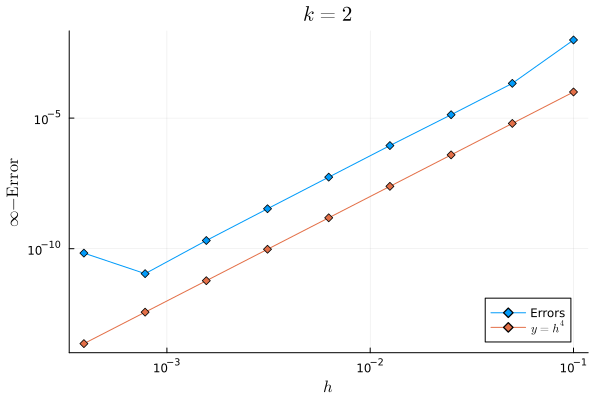
\includegraphics[width=0.48\linewidth]{images/2b1.png}
        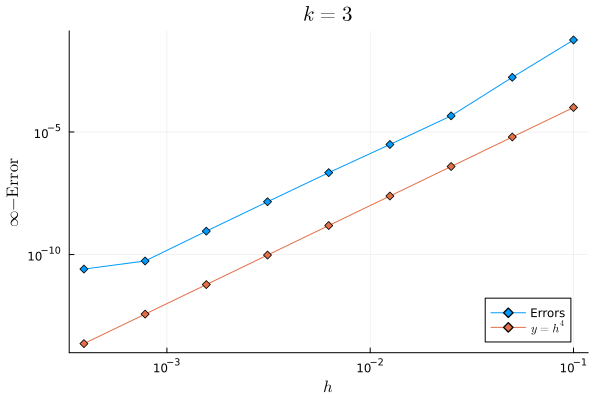
\includegraphics[width=0.48\linewidth]{images/3b1.png}
        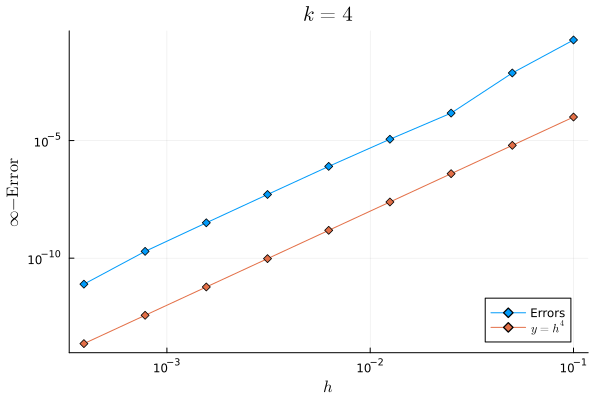
\includegraphics[width=0.48\linewidth]{images/4b1.png}
        \caption{Loglog plots of errors using a fourth-order accurate method for $k \in \{1,2,3,4\}$ compared to a line of slope $h^4$.}
      \end{figure}
    \end{enumerate}
    
    From Figure 2 we can see that the slope of error for reducing grid sizes for $k \in \{1,2,3,4\}$ is order $h^4$ as expected.

\end{solution}

%----------------------------------------------------------------------------------------------------%
%\vskip 20pt
\newpage


\begin{problem}
    Modify the code in {\tt NonlinearBVP.ipynb} to solve
    \begin{align*}
   \begin{cases}
   w'(x) - \epsilon w'''(x) = 0,\\
   w(0) = 0,\\
   w(L) = 0,\\
   w'(L) = 1.
   \end{cases}
    \end{align*}
   Demonstrate the convergence rate by comparing the computed solution
   to the true solution for $\epsilon = 0.1, 0.01$.
\end{problem}

\begin{solution}
  \begin{figure}[h!]
    \centering
    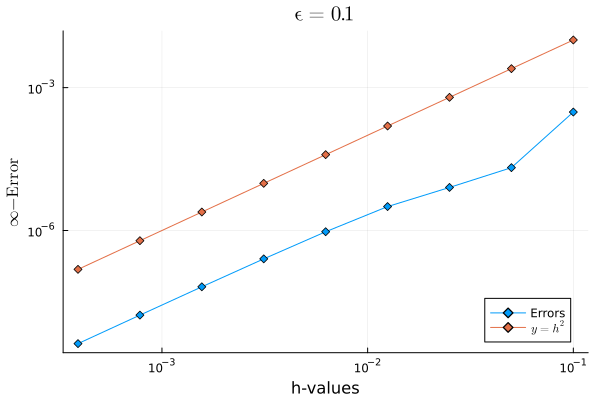
\includegraphics[width=0.48\linewidth]{images/1a2.png}
    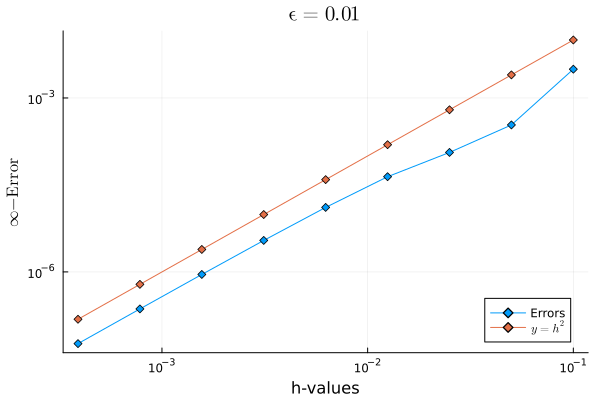
\includegraphics[width=0.48\linewidth]{images/2a2.png}
    \caption{Loglog plots of errors using a second-order accurate method for $\eps \in \{0.1,0.01\}$ compared to a line of slope $h^2$.}
  \end{figure}
  
  From Figure 3 we see that the constructed method for solving the nonlinear BVP is second-order accurate for $\eps \in \{0.1,0.01\}$ when comparing the slope of the error across decreasing step sizes to $y = h^2$. Note, we used $L=1$ in this example.

\end{solution}

\end{document}